\setAuthor{Jaan Kalda}
\setRound{lõppvoor}
\setYear{2012}
\setNumber{G 6}
\setDifficulty{7}
\setTopic{Geomeetriline optika}

\prob{Toru}
Peegeldavate siseseintega toru põhjas on punktvalgusallikas, vt joonist. Toru
sisediameeter on
$d=\SI{12}{mm}$, toru pikkus $l=\SI{60}{mm}$. Vastu toru lahtist otsa on
paigutatud koondav lääts fookuskaugusega $F=\SI{36}{mm}$ ning toru otsast
kaugusele $L=\SI{90}{mm}$ ekraan, millele kinnitatud millimeeterpaberile
on märgitud lõikepunkt optilise peateljega $O$.
Visandage kujutis, mida võib näha ekraanil.

\begin{center}
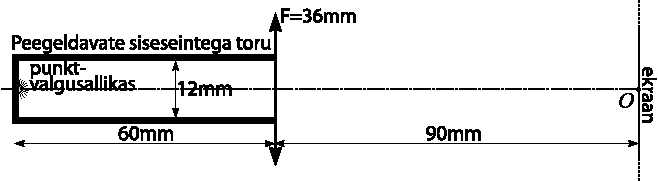
\includegraphics[width=\textwidth]{2012-v3g-06-toru-valgusallikas-lxxts}
\end{center}

\hint
Kui peegeldavate silindriliste seinte asemel oleks kaks tasapeeglit, siis
tekiks optilise peateljega risti punktallika kujutiste lõpmatu jada (peegeldus, peegelduse peegeldus jne). Iga peegeldus tekitaks läbi läätse ekraanil uue kujutise. Tasapeeglite juhtu on võimalik ka silindrilise peegli peale laiendada.

\solu
Kõigepealt paneme tähele, et punktallika kujutis tekib läätsest kaugusele
$$l=\left(\frac 1{36}-\frac 1{60}\right)^{-1}\SI{}{mm}=\SI{90}{mm},$$
st ekraanil. Kui peegeldavate silindriliste seinte asemel oleks kaks tasapeeglit, siis
tekiks punktallika kujutiste lõpmatu jada (peegeldus, peegelduse peegeldus jne), kus 
kahe naaberkujutise vahekaugus on võrdne peeglite vahekaugusega \SI{12}{mm}. 
Läheme nüüd silindrilise juhtumi juurde. Joonise tasandis lebava kiire jaoks on 
kiirekäik täpselt sama, mis tasapeegli puhul, st joonise tasandis tekivad kujutised samuti 
perioodilise rivina, kus kujutiste vahekaugus on \SI{12}{mm}. Joonise tasandit võib pöörata suvaliselt
ümber süsteemi sümmeetriatelje; see tähendab, et kujutised on tegelikult \enquote{laiali määritud} mööda kontsentrilisi
ringjooni raadiustega $n\times\SI{12}{mm}$, kus $n$ on täisarv. Lääts tekitab neist ringidest 
ekraanile $\frac{90}{60}$ korda suurendatud kujutise, 
kus kontsentriliste ringide raadiusteks on $R=n\times \SI{18}{mm}$.

\probeng{Tube}
A tube with reflecting inner walls has a point light source at the bottom of it (see figure). The inner diameter of the tube is $d=\SI{12}{mm}$, the tube’s length is $l=\SI{60}{mm}$. A convex lens with a focal length $F=\SI{36}{mm}$ is placed against the open end of the tube and at a distance $L=\SI{90}{mm}$ from the tip of the tube there is a screen, which has a graph paper attached to it. The intersection point with the optical axis $O$ is marked on the paper. Sketch the image that can be seen on the screen.
\begin{center}
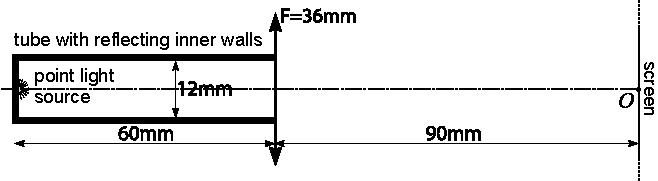
\includegraphics[width=\textwidth]{2012-v3g-06-toru-valgusallikas-lxxts_ing}
\end{center}

\hinteng
If the reflecting cylindrical walls were replaced by two plane mirrors then an infinite sequence of images of the point light source perpendicular to the optical axis would appear (reflection, reflection of the reflection and so on). Each reflection would make a new image on the screen through the lens. The case of plane mirrors can be expanded to examine the cylindrical mirror.

\solueng
Let us first notice that the image of the point light source appears at the following distance from the lens:
$$l=\left(\frac 1{36}-\frac 1{60}\right)^{-1}\SI{}{mm}=\SI{90}{mm},$$ 
meaning on the screen. If there were two plane mirrors in place of the reflecting cylindrical walls then an infinite sequence of the light source’s images would appear (reflection, reflection’s reflection and so on), where the distance between two neighboring images is equal to the distance between the mirrors, 12 mm. Let us now observe the cylindrical case. A ray lying on the plane of the figure has the same path as it would have in the case of a flat mirror, meaning that on the plane of the figure the images also occur in a periodical sequence where the distance between the images is 12 mm. The plane of the figure can be randomly turned around the symmetry axis of the system; this means that the images are actually “smudged” along a concentric circle of radius $n\times\SI{12}{mm}$ where $n$ is an integer. The lens creates a $\frac{90}{60}$ times magnified image of these circles on the screen where the radius of the concentric circles is $R=n\times \SI{18}{mm}$.
\probend